\section{Theoretical Analysis}
\label{sec:analysis}

\paragraph{}
%In this section, we can find the results of each topic required in the theoretical analysis. The numeric results or graphics are presented alongside a short explanation of the interpretation of the problem. All of the results were obatined usig GNU octave and the section is dividid in six different subsections - Subsection ~\ref{subsec:first_topic}, Subsection ~\ref{subsec:second_topic}, Subsection ~\ref{subsec:third_topic}, Subsection ~\ref{subsec:fourth_topic}, Subsection ~\ref{subsec:fifth_topic} and Subsection ~\ref{subsec:sixth_topic} -, one for each topic of the theoretical analysis.

\subsection{Theoretical - Topic I}
\label{subsec:first_topic}

\begin{center}
   \begin{tabular}{|c||c|}
      \hline    
      \multicolumn{2}{|c|} {\bf } \\
      \hline
        \input{}
   \end{tabular}
 \end{center}

 %%%%%%%%%%%%%%%%%%%%%%%%%%%%%%%%%

\subsection{Theoretical - Topic II}
\label{subsec:second_topic}


\begin{center}
   \begin{tabular}{|c||c|}
      \hline    
      \multicolumn{2}{|c|} {\bf } \\
      \hline
        \input{}
   \end{tabular}
 \end{center}
 

 %%%%%%%%%%%%%%%%%%%%%%%%%%%%%%%%%
 
\subsection{Theoretical - Topic III}
\label{subsec:third_topic}

\begin{figure}[H] \centering
\includegraphics[width=0.6\textwidth]{}
\caption{}
\label{}
\end{figure}



 %%%%%%%%%%%%%%%%%%%%%%%%%%%%%%%%%
 
\subsection{Theoretical - Topic IV}
\label{subsec:fourth_topic}

\paragraph{}
The forced response is where the output (the voltage on the capacitor) is going to end up in the long run after all stored energy eventually dissipates. This occors by ignoring the presence of energy storage elements (in our circuit analysis, it ignores the capacitor and its initial voltage, $V_x$). As suggested, plotting the amplitude and phase shift of a sinusoid in a complex plane, we get a complex number in polar form that we can apply to the circuit analysis: a phasor voltage source, $V_s$ = 1. Besides that, we also replaced $C$ with its impedance $Z_C=\frac{1}{\omega C}$.


\[
\left\{\begin{matrix}
f = 1 kHz = 1000 Hz \\
t = 20 ms = 0.020 s \\
\end{matrix}\right.
\]


\begin{center}
   \begin{tabular}{|c||c|}
      \hline    
      \multicolumn{2}{|c|} {\bf Nodal Analysis of Phasors [in Volts]} \\
      \hline
        
 Phasor of Node 1 & 6.12323399574e-17+i1.57079632679e+00 \\ \hline 
 Phasor of Node 2 & 5.78536935465e-17+i1.57079632679e+00 \\ \hline 
 Phasor of Node 3 & 5.10414916043e-17+i1.57079632679e+00 \\ \hline 
 Phasor of Node 5 & 5.83210704339e-17+i1.57079632679e+00 \\ \hline 
 Phasor of Node 6 & 8.26523333807e-02+i-1.42082340747e+00 \\ \hline 
 Phasor of Node 7 & -2.29152014669e-17+i-1.57079632679e+00 \\ \hline 
 Phasor of Node 8 & -3.40788140178e-17+i-1.57079632679e+00 \\ \hline 
   \end{tabular}
 \end{center}
  %%%%%%%%%%%%%%%%%%%%%%%%%%%%%%%%%
 
\subsection{Theoretical - Topic V}
\label{subsec:fifth_topic}

\paragraph{}
The natural response considers the internal initial conditions. The forced response considers the external inputs. Given that, we get the total response by summing the two responses, natural and forced. In fact, this is the principle of superposition in action (in the mathematical sense of differential equations).

\[
\left\{\begin{matrix}
v_t=v_n+v_f\\
f = 1 kHz = 1000 Hz \\
\end{matrix}\right.
\]

\begin{figure}[H] \centering
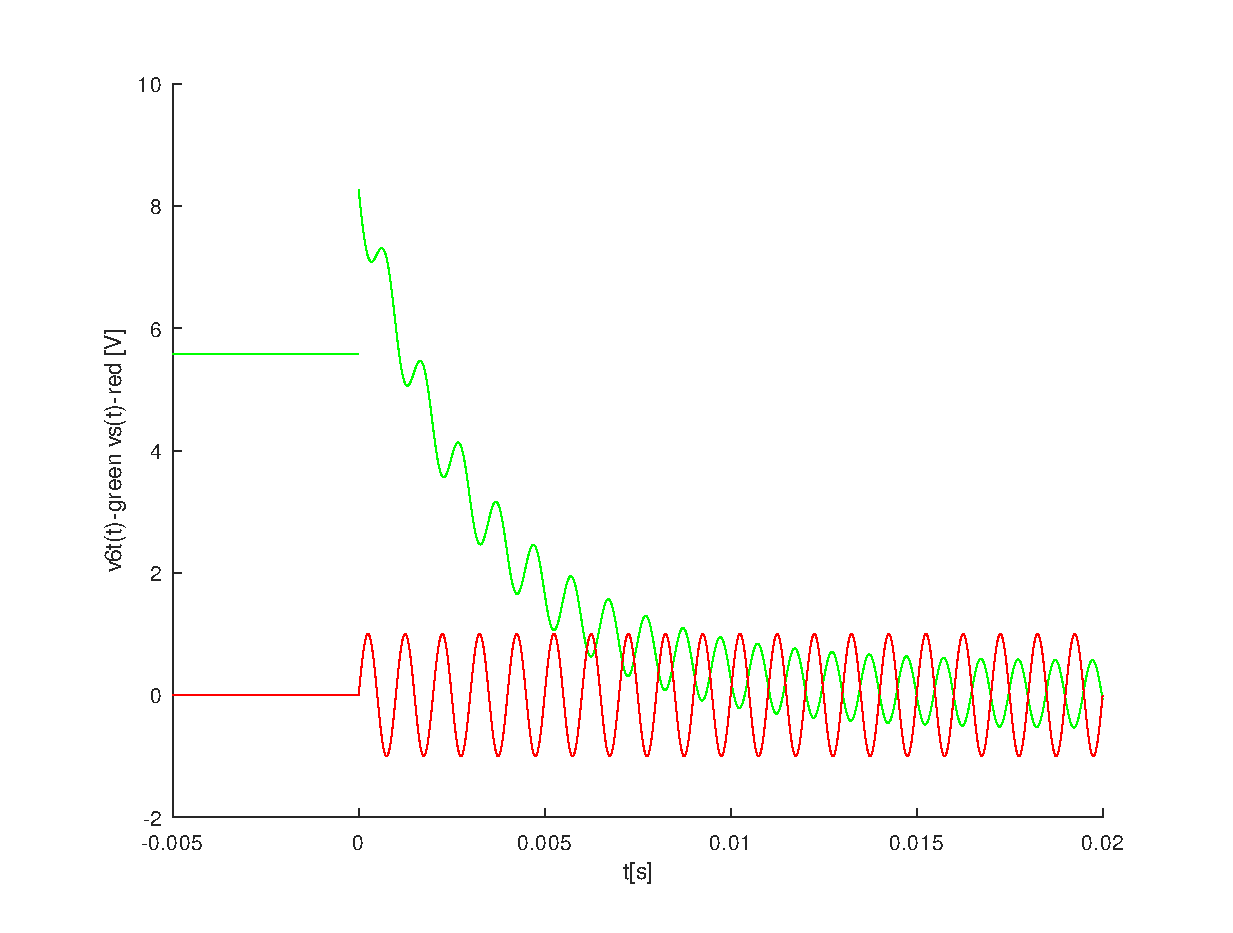
\includegraphics[width=0.6\textwidth]{total.eps}
\caption{The final total solution, $V6(t)$,  and $v_s(t)$ during time interval [-5, 20] ms.}
\label{fig:theo_fifth}
\end{figure}


Where $t$ is expressed in seconds (s) along the x-axis and 
$V6(t)$, the total solution, and $v_s$ are expressed in Volts (V) along the y-axis.

In the graphic above, it is ineteresting to note that, while the voltage emited by the source $V_s$ is constant, the node 6 will also have a constant voltage. This is because for $t<0$ the circuit will essentially behave as one of continuos current. After this time mark, the circuit reveals its alternate current nature and both the voltages of the source and of node 6 will vary sinousoidally.



  
  %%%%%%%%%%%%%%%%%%%%%%%%%%%%%%%%%

\subsection{Theoretical - Topic VI}
\label{subsec:sixth_topic}

\paragraph{}In this subsection, an analysis of the variation of the magnitude and phase of the phasors of $V_c$ $V_6$ and $V_s$ is made in function of the frequency. The first graphic presents the study of the variation of the magnitude and the second the study of the fase. In both graphics, the frequency $f$ in the x-axis varies from 0.1Hz to 1MHz


\[
\left\{\begin{matrix}
f =\in [0.1 , 1] MHz \\
v_c(f)=v_6(f)-v_8(f) \\
\end{matrix}\right.
\]


\begin{figure}[H] \centering
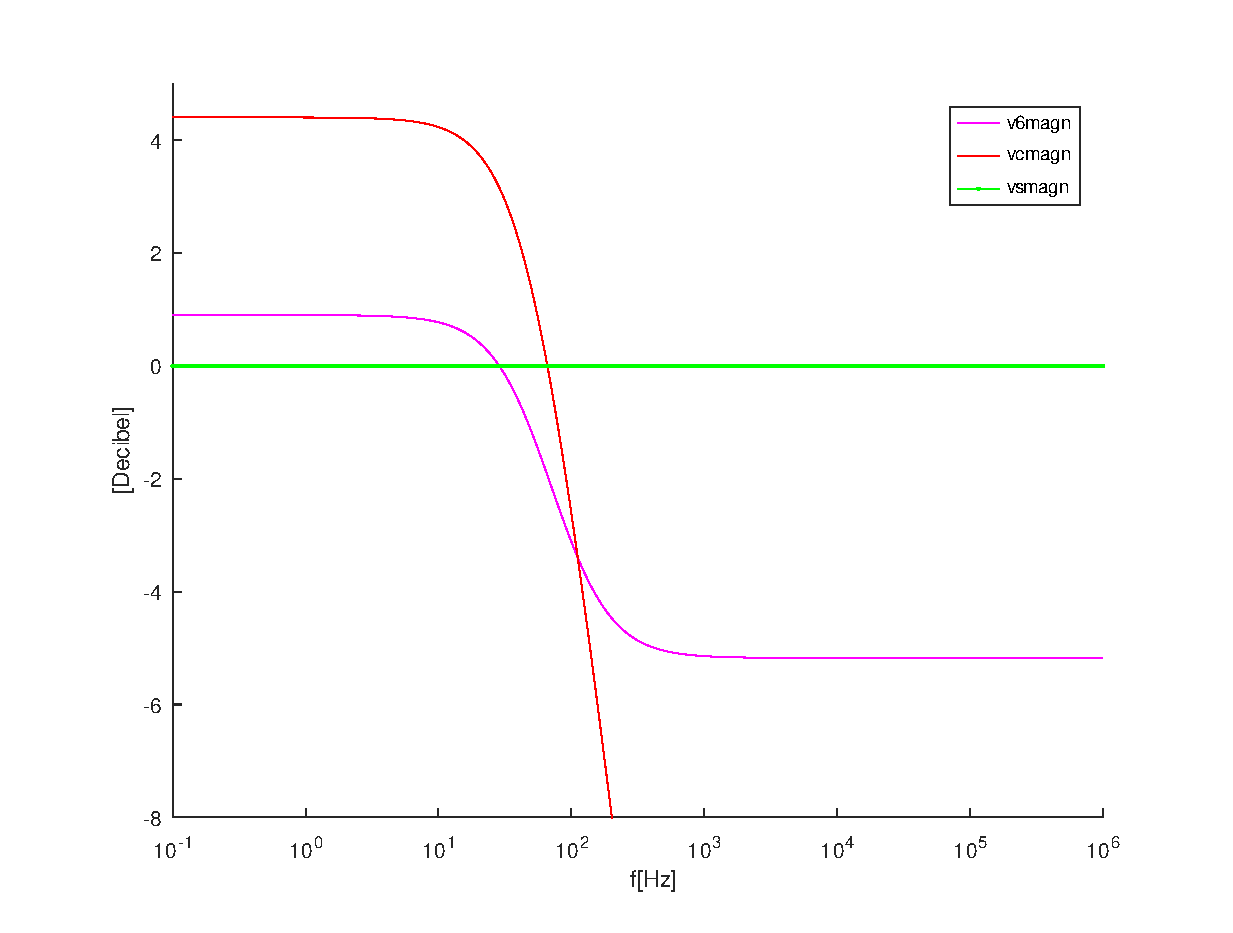
\includegraphics[width=0.6\textwidth]{magnitude.eps}
\caption{Magnitude of $v_s(f)$,  $v_c(f)$  and $v_6(f)$ during frequency interval [0.1 , 1] MHz.}
\label{fig:magnitudetheo}
\end{figure}

The frequency $f$ is expressed in Hertz (Hz) along the x-axis and 
the magnitude of $v_s(f)$,  $v_c(f)$  and $v_6(f)$ is expressed with a logscale decibel (dB) along the y-axis.\\ \\
When looking at this graph, a couple of things are important to highlight. First, $V_s$ will always have magnitude 0 because, given that its absolute value is 1 and we are using a logscale, $log(1)=0$. Second, we also note that the $v_c$ graph line does not resemble the one that represents $v_6$. This is because the voltage of the node 8 will also vary. 


\begin{figure}[H] \centering
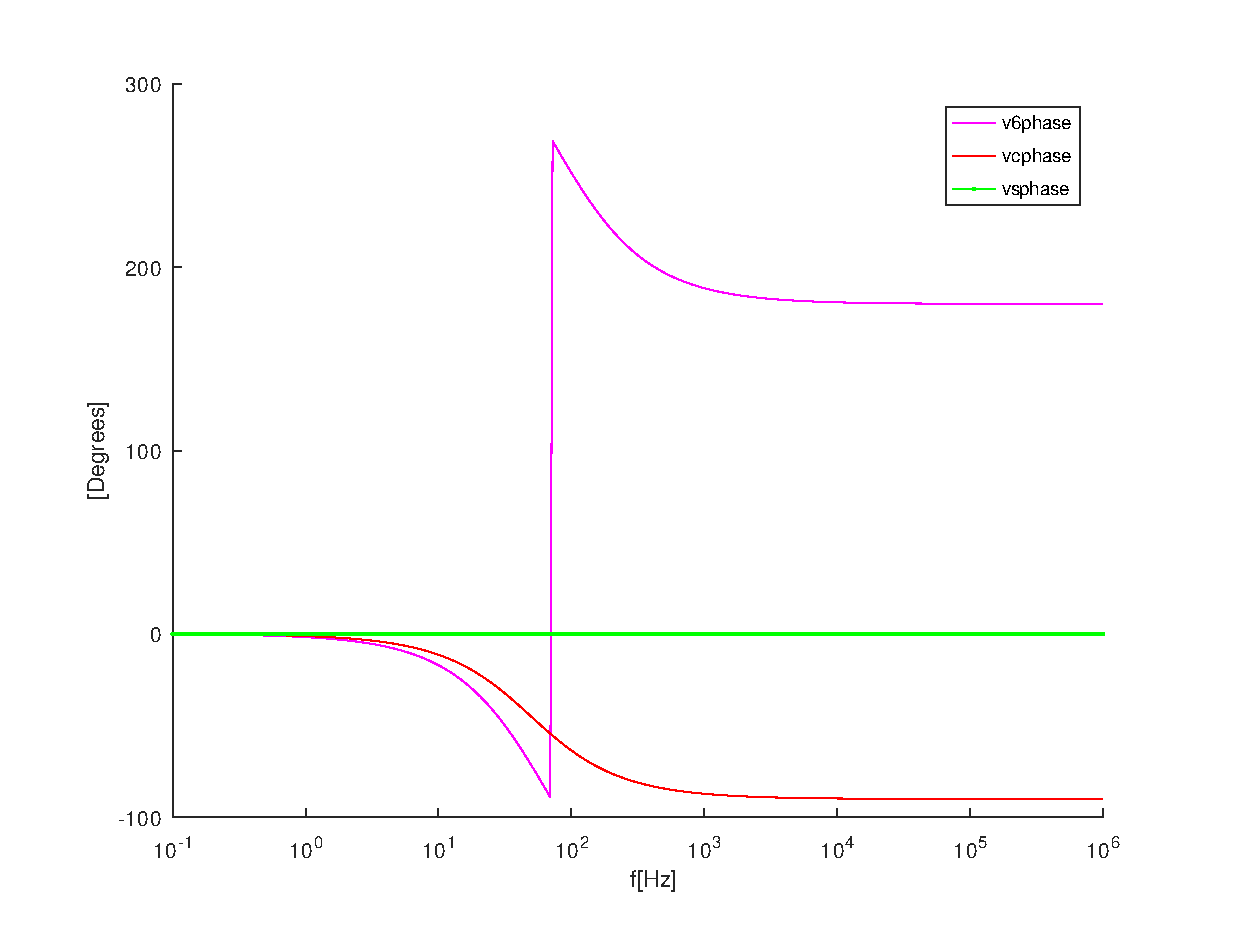
\includegraphics[width=0.6\textwidth]{phase.eps}
\caption{Phase $v_s(f)$,  $v_c(f)$  and $v_6(f)$ during frequency interval [0.1 , 1] MHz.}
\label{fig:phasetheo}
\end{figure}

The frequency $f$ is expressed in Hertz (Hz) along the x-axis and
the phase of $v_s(f)$,  $v_c(f)$  and $v_6(f)$ is expressed in degrees along the y-axis.\\ \\
In this graph, the first thing that comes to the eye is the fact that the phase of $V_s$ will always be constant and that, once again, the $v_c$ graph line does not resemble the one that represents $v_6$. 

